\section{Modeling and Control}\label{section_modelcontrol}

To plan a strategy for controlling the tension and the length of the \scpsnospace, their physical characters must be modeled with mathematical equations. Behaviors of the \scps were modeled with linear equations, and this led to the equations of \antanospace.
As a result, control strategies for \apc was established.

\subsection{Modeling of the \ANTA}\label{section_thermo_model}
\scp can be expressed as a combination of a mechanical model and a thermal constant. The correlation between muscle's displacement $x$, temperature $T$, elastic constant $k$, damping constant $b$, thermal constant $c$ and tension $F$ is shown in \eqref{thermo-mechanical_model} \cite{yip}.
(Figure \ref{ModelMus})
\begin{equation} \label{thermo-mechanical_model}
F=k(x-x_0) + b\dot{x}+c(T-T_0)
\end{equation}
Also, by considering the Newton's cooling law, the correlation between specific heat $C_{th}$ and thermal conductivity $\lambda$ can be expressed as \eqref{thermo-electrical_model} \cite{yip}.

\begin{equation} \label{thermo-electrical_model}
C_{th}\frac{dT(t)}{dt} = P(t) - \lambda(T(t)-T_{ambient})
\end{equation}

Since the \anta is a sum of two \scpsnospace, the displacement of two \scps is complementary(Figure \ref{ModelAnt}). If one of the muscle's displacement is expressed as $x$, another becomes $-x$. By considering $x=r\theta$ and $\tau=J\ddot{\theta}$, arm's equation of a motion is shown in \eqref{EqAnta}, where $r$, $\theta$, $\tau$ and $J$ are radius of arm, rotational displacement, torque and moment of inertia, respectively.
(Figure \ref{ModelAnt})
\begin{gather}
\tau = [-kx-b\dot{x}+c(T_1-T_0) - (kx+b\dot{x}+c(T_2-T_0))]r. \nonumber \\
\therefore J\ddot{\theta}+2br^2\dot{\theta}+2kr^2\theta = cr(T_1-T_2). \label{EqAnta}
\end{gather}

\begin{figure}[t]
	\centering
	\begin{subfigure}[t]{0.2\textwidth}
		\centering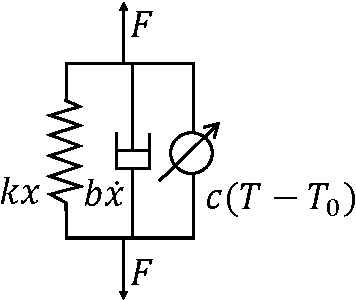
\includegraphics[width=\textwidth]{Model_muscle-cropped_compatible.pdf}
		%\centering\includegraphics[width=\textwidth]{example-image-a}
		\caption{\label{ModelMus}}
	\end{subfigure}
	\begin{subfigure}[t]{0.31\textwidth}
		\centering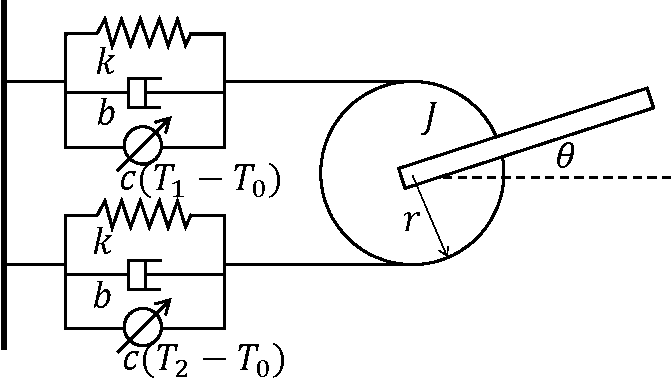
\includegraphics[width=\textwidth]{Model_anta-cropped_compatible.pdf}
		%\centering\includegraphics[width=\textwidth]{example-image-a}
		\caption{\label{ModelAnt}}
	\end{subfigure}
	\caption[Modeling of the \scps and \anta]{\subref{ModelMus} The \scps can be expressed as a combination of a spring, damper, and temperature-dependent system. \subref{ModelAnt} The \anta can be expressed with two complimentary muscles, which change the angular position.}
	\label{model}
\end{figure}



\subsection{Basic Strategy for the \APC}

Based on mathematical modeling of the \scpsnospace, their control strategies and results are shown. Also, the \anta was controlled to follow the desired position, which is a function of time. This management will be called as `\apcnospace'.

By assuming that $\ddot{\theta}$ and $\dot{\theta}$ are small enough, we could observe correlation between $\theta$ and $T_{1}$, $T_{2}$ from \eqref{EqAnta} as \eqref{simple_assume}.
\begin{equation} \label{simple_assume}
\theta = \frac{c}{2kr}(T_{1}-T_{2}).
\end{equation}
By multiplying Laplace transformed equations of \eqref{thermo-electrical_model} and \eqref{simple_assume}, transfer function of $P$ and $\theta$ was discovered as \eqref{apc_transfer}.

\begin{equation} \label{apc_transfer}
\frac{\theta(s)}{P(s)} = \frac{c/2kr}{C_{th}s+\lambda}.
\end{equation}
Therefore, the process of controlling $\theta$ into $\theta_{ref}$ by applying constant power can be shown as block diagram in figure \ref{AntaControl_constant}. 

In this situation, $K_{\theta,P}$ is constant. By applying constant power to only one of the muscles, $\theta$ at steady state was measured. Linear fitting of figure \ref{KthetaP} gave us the following constant.

\begin{equation}
K_{\theta,P} = \SI{0.185}{\watt\per\degree}. \nonumber
\end{equation}
For the fast and precise control, a lead compensator was added and subsequently, feedback, and feedforward control were applied, as can be seen in figure \ref{position_open_loop}, \ref{position_closed_loop}.

\begin{figure}[t]
	\centering
	\begin{minipage}{0.30\textwidth}
		\begin{subfigure}{\linewidth}
			\centering
			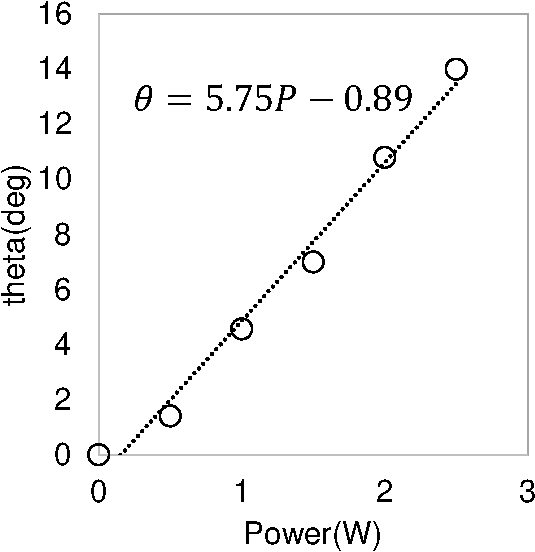
\includegraphics[width=\linewidth]{K_theta_P_v4-cropped.pdf}
			\caption{\label{KthetaP}}
		\end{subfigure}
	\end{minipage}%
	\begin{minipage}{0.6\textwidth}
		\centering
		\begin{subfigure}{0.55\linewidth}
			\centering
			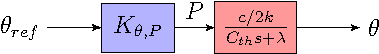
\includegraphics[width=\linewidth]{Diagram(v4)_position_constant.pdf}
			\caption{\label{AntaControl_constant}}
		\end{subfigure}
		
		\begin{subfigure}{0.73\linewidth}
			\centering
			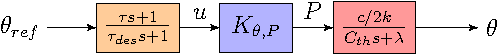
\includegraphics[width=\linewidth]{Diagram(v4)_position_openloop.pdf}
			\caption{\label{position_open_loop}}
		\end{subfigure}
		
		\begin{subfigure}{\linewidth}
			\centering
			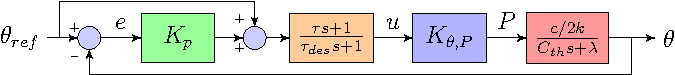
\includegraphics[width=\linewidth]{Diagram(v4)_position_feedback.pdf}
			\caption{\label{position_closed_loop}}
		\end{subfigure}
	\end{minipage}
	\caption[Block diagrams for the \apc]{\subref{KthetaP} There's a linear relationship between applied power and $\theta$ at steady state. \subref{AntaControl_constant} Process of obtaining desired angle with constant power. \subref{position_open_loop} Process of the \apc including a lead compensator. \subref{position_closed_loop} Process of the \apc including feedback and feedforward.}
	\label{anta_position_diagrams}
\end{figure}


\subsection{Antagonistic Position Control Strategy}
In this section, we aim to make a simple sin wave motion of the \anta as \eqref{theta_ref}. By doing this, we could check the possibility of the \apc for any complicated motion. Basically, according to the equation \eqref{simple_assume}, we could increase $\theta$ by heating muscle 1 and decrease $\theta$ by heating muscle 2. Therefore, strategy shown in Table.\ref{table_apc_basic} was used.

\begin{equation}\label{theta_ref}
\theta_{ref}(t)=(\SI{9}{\degree})\sin(2\pi 0.025t)
\end{equation}

\begin{table}[t]
	\caption{Basic strategy for the \apc.}
	\label{table_apc_basic}
	\begin{center}
		\begin{tabular}{c||c|c|c|c}
			\hline
			Time(s) & 0-10 & 10-20 & 20-30 & 30-40 \\
			\hline
			Muscle 1 & Heat & Keep & Keep & Heat \\
			Muscle 2 & Keep & Heat & Heat & Keep \\
			\hline
			$\theta$ & increase & decrease & decrease & increase \\
			\hline
		\end{tabular}
	\end{center}
\end{table}

Since the Laplace transformation of \eqref{theta_ref} is too complicated, 
it was approximated as \eqref{theta_ref_approx} by dividing \eqref{theta_ref} into 12 steps. In this case, demanded power can be calculated as \eqref{power_derived} since $n=12$. 
\footnote{In equation \eqref{power_derived}, $\theta_{ref,pre}$ is a value of $\theta_{ref}$ in the previous step. Also, $t$ is elapsed time after starting a new step.}
\footnote{$U(t)$ is unitary step function.}
\begin{equation} \label{theta_ref_approx}
\begin{aligned} 
%\theta_{ref}(t) = \sum_{i=0}^{n-1}{(\theta_{ref,i+1}-\theta_{ref,i})U(t-i\Delta T)} 
\theta_{ref}(t) & = \sum_{i=0}^{n-1}{(\theta_{ref,i+1}-\theta_{ref,i})U(t-i\Delta T)} \\
& = \sum_{i=0}^{n-1}{\left(\sin{\frac{2(i+1)\pi}{n}}-\sin{\frac{2i\pi}{n}}\right)U\left(t-40\frac{i}{n}\right)}. \\
\end{aligned}
\end{equation}

\begin{equation} \label{power_derived}
P(t)=\theta_{ref}K_{\theta,P}\left(1+\left(\frac{\theta_{ref}-\theta_{ref,pre}}{\theta_{ref}}\right)\left(\frac{\tau}{\tau_{des}}-1\right)e^{-\frac{t}{\tau_{des}}}\right).
\end{equation}


%% TODO : sustainable 로 들어가는 문장이 필요함. 딱히 subsection을 새로 만드는 것보다는 문장으로 연결하는게 나을듯.

%\subsection{Sustainable Antagonistic Position Control Strategy}\label{section_simulation}
%The method for making sin wave motion was discussed previously. 
However, since the temperature of the muscles in the initial state and final state is significantly different, the strategy shown in table \ref{table_apc_basic} won't be sustainable. In other words, \scps will be overheated and break down.
Therefore, we needed to make the temperature of the initial state and final state the same. This was performed by cooling the muscle during the last 1/4 period of sin wave, as shown in Table \ref{table_apc_sustain}.

\begin{table}[t]
	\caption{Sustainable \apc strategy.}
	\label{table_apc_sustain}
	\begin{center}
		\begin{tabular}{c||c|c|c|c|c|c|c}
			\hline
			Time(s) & 0 & 0-10 & 10-20 & 20-30 & \multicolumn{2}{|c|}{30-40} & 40 \\
			\hline
			Muscle 1 & $T_0$ & Heat & Keep & Keep & Weakly Cool & Heat & $T_0$ \\
			Muscle 2 & $T_0$ & Keep & Heat & Heat & Strongly Cool & Keep & $T_0$ \\
			\hline
			$\theta$ & $0^{\circ}$ & increase & decrease & decrease & \multicolumn{2}{|c|}{increase} & $0^{\circ}$ \\
			\hline
		\end{tabular}
	\end{center}
\end{table}